\documentclass[a4paper]{article}
\usepackage{a4wide}
\usepackage[utf8]{inputenc}
\usepackage[ngerman]{babel}
\usepackage{amsmath}
\usepackage{graphicx}
\usepackage{listings}

\title{Praktikum „Integritätsbedingungen“, Phase 1}
\author{Henning Basold \and Igor Zerr}
\date{\today}
\begin{document}
\maketitle
\section{Modell}
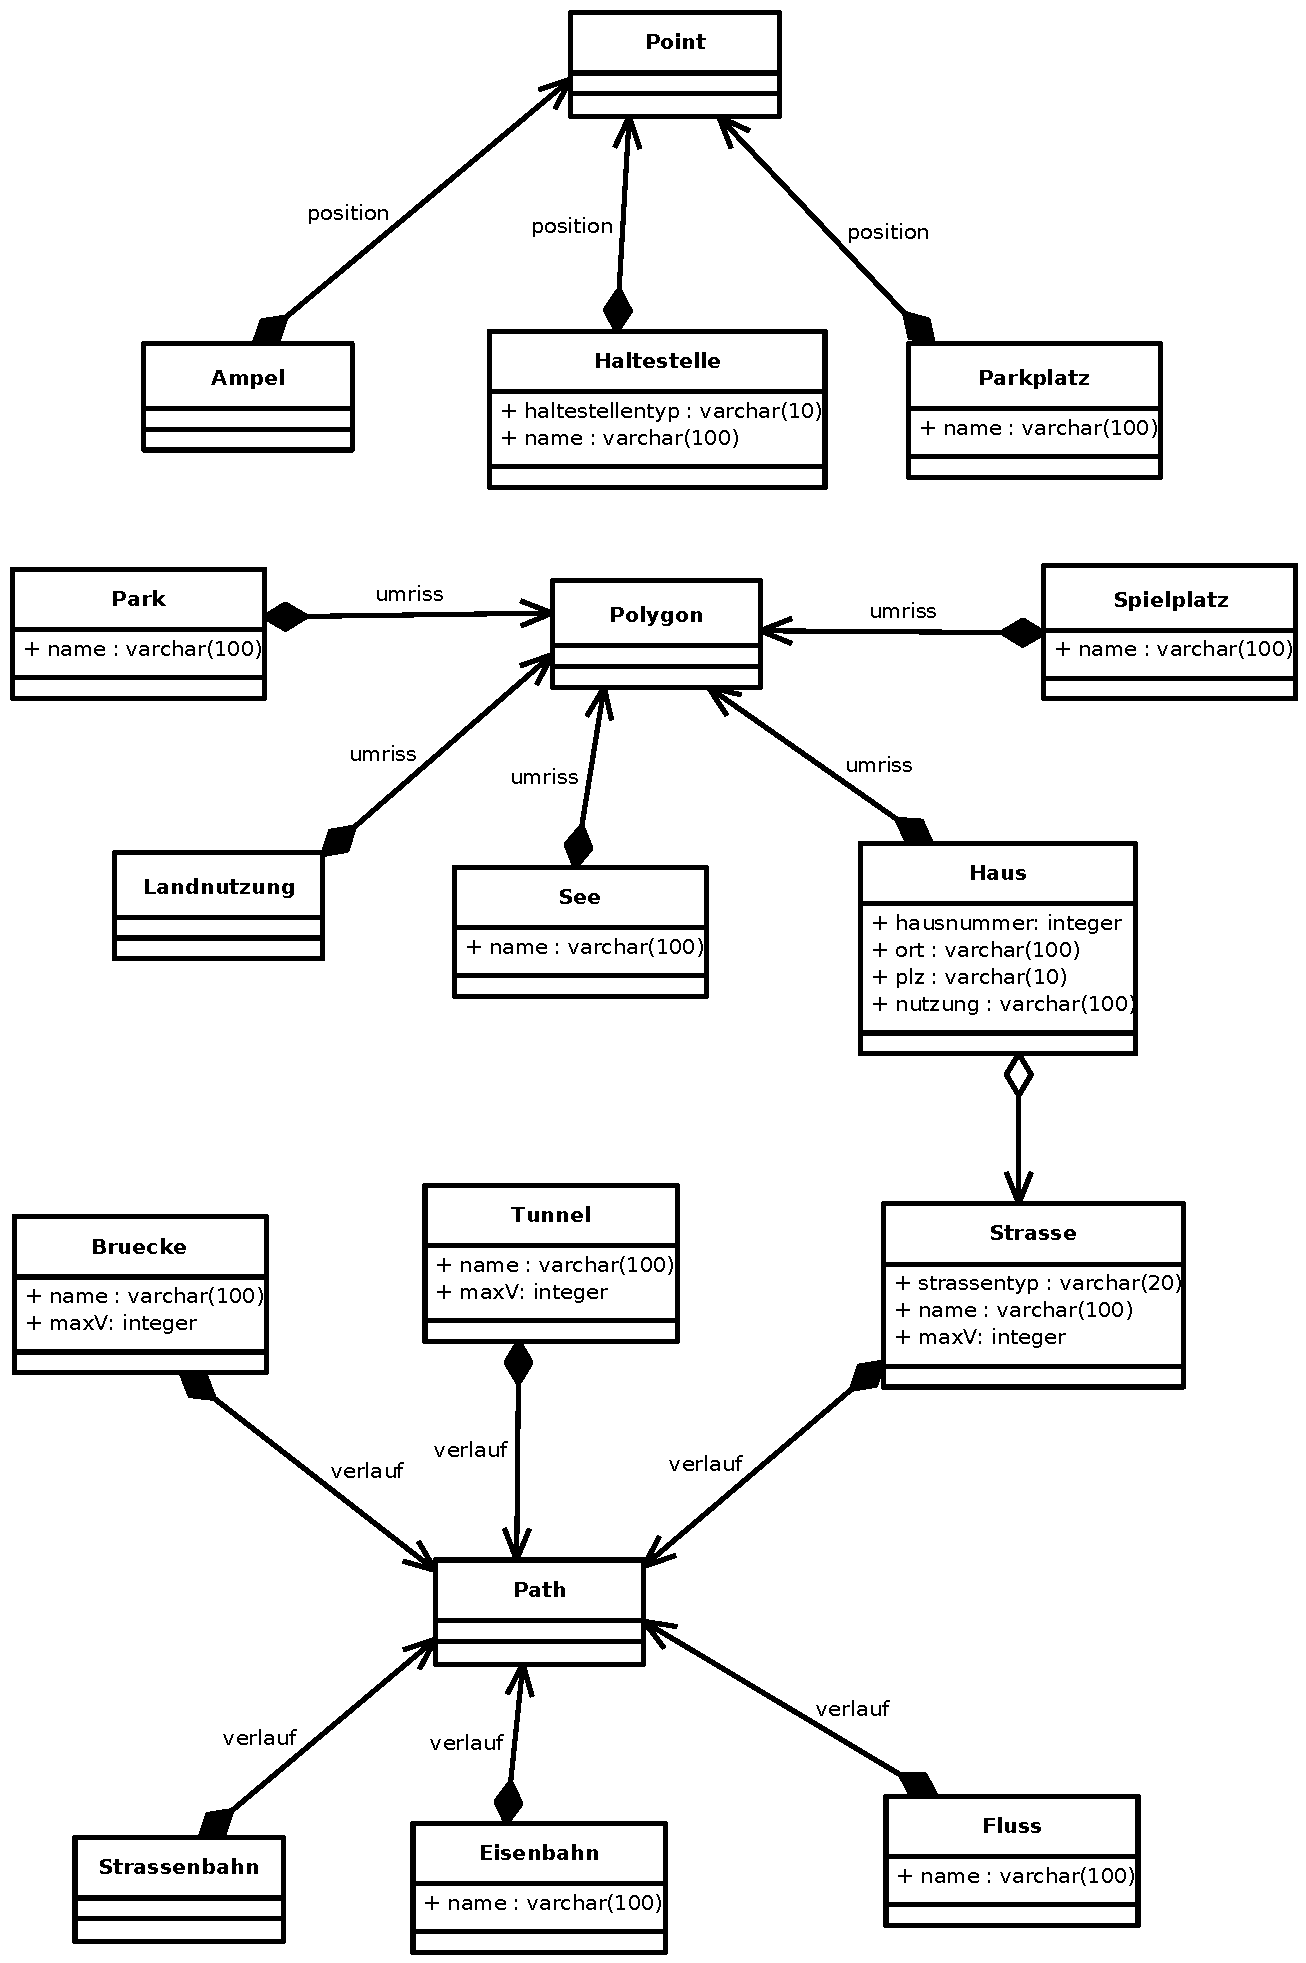
\includegraphics[width=\textwidth,keepaspectratio]{Model/model.pdf}

\section{Relationsschemata}
\lstinputlisting[language=SQL,breaklines=true]{Relationschemata.txt}

\section{Assertions}
\begin{enumerate}
    \item (innere) Punkte disjunkt bei
    \begin{enumerate}
        \item HOUSE\_STREET\_DISJOINT: Haus $\longleftrightarrow$ Straße
        \item HOUSE\_HOUSE\_DISJOINT: Haus $\longleftrightarrow$ Haus
        \item HOUSE\_LAKE\_DISJOINT: Haus $\longleftrightarrow$ See
        \item STREET\_LAKE\_DISJOINT: Straße $\longleftrightarrow$ See
        \item STREET\_LANDUSE\_DISJOINT: Straße $\longleftrightarrow$ Landnutzung
        \item STREET\_PLAYGROUND\_DISJOINT: Straße $\longleftrightarrow$ Spielplatz
    \end{enumerate}
    
    \item NO\_STANDALONE\_STOP: An einer Haltestelle verläuft eine Straße,
        Straßenbahn- oder Eisenbahnlinie in höchstens Abstand r
    \item WATER\_CROSSING: Wenn eine Straße, Straßenbahn- oder Eisenbahnlinie und ein Fluss sich kreuzen,
        ist dort eine Brücke oder ein Tunnel über/unter dem Fluss
    \item TRAFFIC\_LIGHT\_AT\_STREET: Ampeln stehen an Straßen mit höchstens Abstand r
    \item PARKING\_REACHABLE: Zu einem Parkplatz führt eine Straße oder an diesem in höchstens Abstand r entlang
\end{enumerate}

\lstinputlisting[language=SQL]{assertions.txt}

\subsection{Bemerkungen}
Leider konnten wir die jeweiligen Radien noch nicht feststellen. Dazu müssen wir erst die Daten
analysieren, um einen vernünftigen Wert zu erhalten.

Die Funktion „approx\_circle“ stellt einen Kreis angenähert als Pfad dar. Dies ist nötig, da kein Schnitt
zwischen Kreisen und Pfaden in Postgresql direkt möglich ist.
\end{document}
